% Copyright 2009 by Joyan <joyanlj@gmail.com>.
% Last Modified Feb. 20, 2009
%
% In principle, this file can be redistributed and/or modified under
% the terms of the GNU Public License, version 2.
%
% However, this file is supposed to be a template to be modified for
% your own needs. For this reason, if you use this file as a template
% and not specifically distribute it as part of a another
% package/program, I grant the extra permission to freely copy and
% modify this file as you see fit and even to delete this copyright
% notice.

\documentclass[a4paper,dvipdfm]{ctexart}
%\usepackage{indentfirst}%用于首行缩进
%\usepackage[width=500pt]{geometry}%用于设置页面大小
\usepackage{listings}%用于提供lstlisting代码显示环境
\usepackage[dvipdfm]{graphicx}
\usepackage[usenames,dvipsnames]{color}
\usepackage{xcolor}
%\usepackage{threeparttable}%用于表格内注释
%\usepackage[centerlast]{caption2} %浮动图形和表格标题样式
%\usepackage[rightcaption]{sidecap}%轻松的得到标题在一边的浮动图形或表格
%\usepackage{colortbl}%彩色表格
%\usepackage{multirow}%排版表格里的跨行文本数据和对齐方式
%\usepackage{textcomp}%常见数理单位和货币符号
%\usepackage[section]{placeins}%立即处理浮动体,section选项要求浮动体在它们所在的章节中排出
%\usepackage{subfigure} %%图形或表格并排排列

% \usepackage{fancyhdr}%设置页眉页脚
% \fancypagestyle{plain}{%
%   \fancyhf{}              
%   \fancyhead[R]{\thepage}
%   \fancyhead[L]{00648333}
% }
% \fancyhead[R]{\thepage}
% \fancyhead[L]{00648333}
% \pagestyle{fancy}

% \usepackage{setspace}%设置行距
% \doublespacing%双倍行距

% \usepackage[dvipdfm,a4paper,CJKbookmarks,bookmarks=true,bookmarksopen=true]{hyperref}%很强大的一个东西
% \hypersetup{
%     pdftitle={},
%     pdfauthor={Wen Zhang},
%     pdfkeywords={},
%     bookmarksnumbered,
%     pagebackref=true,
%     breaklinks=true,
% %    pdfview=FitH,       % Or try pdfstartview={FitV}, This lead to uncorrect bookmarks
%     urlcolor=cyan,
%     colorlinks=true,
%     citecolor=magenta,          %citeref's color
%     linkcolor=magenta,
%         }



\DeclareGraphicsExtensions{.eps,.ps,.eps.gz,.ps.gz,.eps.Z,.EPS,.pdf,.PDF}%声明图片后缀

\newcommand{\upcite}[1]{\textsuperscript{\cite{#1}}} %自定义命令\upcite, 使参考文献引用以上标出现

\graphicspath{{figures/}}

\makeatletter
\newenvironment{tablehere}
  {\def\@captype{table}}
  {}

\newenvironment{figurehere}
  {\def\@captype{figure}}
  {}
\makeatother



\begin{document}
%  ABAP (R/2 4.3, R/2 5.0, R/3 3.1, R/3 4.6C, R/3 6.10)
% ACSL                               Ada (83, 95)
% Algol (60, 68)                     Assembler (x86masm)
% Basic (Visual)                     C (ANSI, Objective, Sharp)
% C++ (ANSI, GNU, ISO, Visual)       Caml (light, Objective)
% Clean                              Cobol (1974, 1985, ibm)
% Comal 80                           csh
% Delphi                             Eiffel
% Elan                               erlang
% Euphoria                           Fortran (77, 90, 95)
% GCL                                Haskell
% HTML                               IDL (empty, CORBA)
% Java (empty, AspectJ)              ksh
% Lisp (empty, Auto)                 Logo
% make (empty, gnu)                  Mathematica (1.0, 3.0)
% Matlab                             Mercury
% MetaPost                           Miranda
% Mizar                              ML
% Modula-2                           MuPAD
% NASTRAN                            Oberon-2
% OCL (decorative, OMG)              Octave
% Pascal (Borland6, Standard, XSC)   Perl
% PHP                                PL/I
% POV                                Prolog
% Python                             R
% Reduce                             Ruby
% S (empty, PLUS)                    SAS
% Scilab                             SHELXL
%                                    SQL
% Simula (67, CII, DEC, IBM)
% tcl (empty, tk)
% TeX (AlLaTeX, common, LaTeX, plain, primitive)
% VBScript                           Verilog
% VHDL (empty, AMS)                  VRML (97)
% XML
\lstset{
  language={C},
  linewidth=0.8\textwidth{},
  breaklines=true,
  numbers=none,
  numberstyle=\small{},
  stepnumber=5,
  numbersep=5pt,
  columns=fullflexible,
  basicstyle=\normalsize{}\ttfamily{},          % print whole listing small
  backgroundcolor=\color{black!10!white},
  frame=leftline,
  emph={czj,joyan},
  emphstyle=\color{blue}\bfseries,
  keywordstyle=\color{blue}\bfseries,
  identifierstyle=\color{black},           % nothing happens 
  escapeinside=`',
  commentstyle=\color{black}, % white comments
  stringstyle=\ttfamily,      % typewriter type for strings
  showstringspaces=false}     % no special string spaces

%%%%%%%%%%%%%%%%%%%%%%%%%%% 正文开始 %%%%%%%%%%%%%%%%%%%%%%%%%%%%%%


\title{计算机体系结构实习二}
\author{陈志杰\\00648333\\chenzhijie@icst.pku.edu.cn}
\date{}

\maketitle
  
\section{指令系统的设计}

为了完成插入排序的功能,该指令系统需要 add, addi, lw, sw, slt, beq, bne 和
swi 等指令,其功能可以类比 MIPS 指令系统中类似指令的功能,现分别介绍其
详细信息如下:

\textbf{声明:本实验指令系统中add、addi、lw和sw定义取自实习中所给
  的demo(addi做了简单改进以支持带符号立即数加法),在后面的其他指令设
  计中尽量做到与现有指令格式一致。}

\subsection{ADD 加法指令}
\label{sec:add-}

指令助记符、格式等见表\ref{tab:add}.

\begin{table}[hbt!]
  \centering
  \begin{tabular}{|l|l|l|l|l|l|}
    \hline
    &add&RD&RS&RT&\\
    \hline
    bit&31-26&25-21&20-16&15-11&10-0\\
    \hline
    &000001&*****&*****&*****&00000000000\\
    \hline
  \end{tabular}
  \caption{ADD 加法指令}
  \label{tab:add}
\end{table}

\textbf{由于add、addi、lw、sw是实习要求的demo部分提供的,因此在此不全
  部列出其详细格式。下面是我自己添加的slt、beq和bne指令的格式:}

\subsection{slt 比较并设置指令}
\label{sec:slt-}

slt 的指令助记符、格式等如表\ref{tab:slt}.

\begin{table}[hbt!]
  \centering
  \begin{tabular}{|l|l|l|l|l|l|}
    \hline
    &add&RD&RS&RT&\\
    \hline
    bit&31-26&25-21&20-16&15-11&10-0\\
    \hline
    &001011&*****&*****&*****&00000000000\\
    \hline
  \end{tabular}
  \caption{SLT 比较并设置指令}
  \label{tab:slt}
\end{table}

SLT 的功能与 MIPS 中定义一致,即比较 RS域指示的寄存器值是否小于 RT域指
示的寄存器值并将结果存入 RD域指示的寄存器。

\subsection{BEQ 条件跳转指令}
\label{sec:beq-}

beq 的指令助记符、格式等如表\ref{tab:beq}.

\begin{table}[hbt!]
  \centering
  \begin{tabular}{|l|l|l|l|l|}
    \hline
    &beq&RD&RS&16-IMME\\
    \hline
    bit&31-26&25-21&20-16&15-0\\
    \hline
    &001100&*****&*****&****************\\
    \hline
  \end{tabular}
  \caption{BEQ 条件跳转指令}
  \label{tab:beq}
\end{table}

beq 指令的功能与 MIPS 中定义的类似,即比较 RD 域指示的寄存器和 RS 域指
示的寄存器的值是否相等,若相等则跳转。

\subsection{BNE 条件跳转指令}
\label{sec:bne-}

bne 的指令助记符、格式等如表\ref{tab:bne}.

\begin{table}[hbt!]
  \centering
  \begin{tabular}{|l|l|l|l|l|}
    \hline
    &bne&RD&RS&16-IMME\\
    \hline
    bit&31-26&25-21&20-16&15-0\\
    \hline
    &001101&*****&*****&****************\\
    \hline
  \end{tabular}
  \caption{BNE 条件跳转指令}
  \label{tab:bne}
\end{table}

bne 指令的功能与 MIPS 中定义的类似,即比较 RD 域指示的寄存器和 RS 域指
示的寄存器的值是否相等,若不相等则跳转。

\section{数据通路的设计}
\label{sec:datapath}

本指令系统的数据通路如图\ref{fig:datapath}.本图源自课本,与课本不同的
地方主要是图中间通向寄存器堆的三条线的定义以及寄存器堆中 Write
Register 和 Read Register 2 的位置。

\begin{figure}[hbt!]
  \centering
  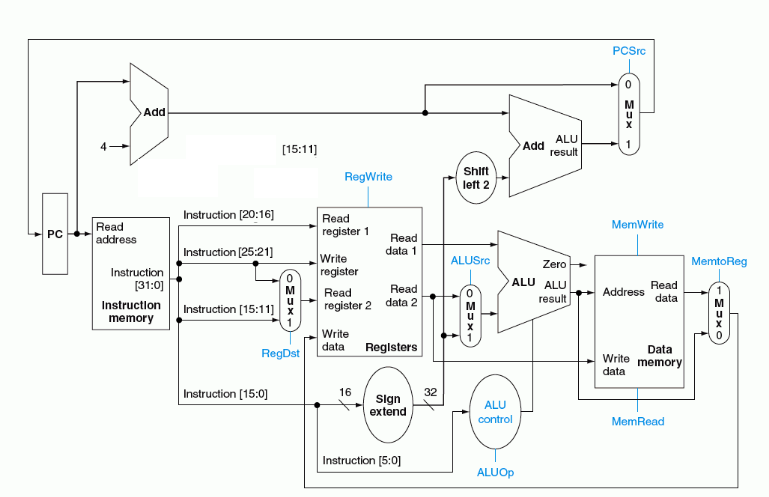
\includegraphics[width=1.2\textwidth]{datapath.png}
  \caption{数据通路示意图}
  \label{fig:datapath}
\end{figure}

各控制信号意义如下:
\begin{description}
\item[PCSrc] PC寄存器更新的来源:是只递增还是递增后还要加一个便宜;
\item[RegDst] 寄存器堆二号数据输出线路上是读的RD的值还是RT的值;
\item[RegWrite] 控制是否向寄存器堆写入数据;
\item[ALUSrc] 控制ALU的第二个参数由谁提供;
\item[ALUOp] 控制ALU是进行什么操作;
\item[MemWrite] 控制是否写存储器;
\item[MemRead] 控制是否读存储器;
\item[MemtoReg] 控制向寄存器写入的数据来自存储器还是ALU
\end{description}

各个控制信号在不同时期的值见表\ref{tab:dc}。

\begin{table}[hbt!]
  \centering
  \begin{tabular}{|l|l|l|l|l|l|l|l|l|}
    \hline
    Inst&PCSrc&RegDst&RegW&ALUSrc&ALUOp&MemW&MemR&Mem2Reg\\
    \hline
    add&0&1&1&0&+&0&0&0\\
    addi&0&*&1&1&+&0&0&0\\
    lw&0&*&1&1&+&0&1&1\\
    sw&0&0&0&1&+&1&0&*\\
    slt&0&1&1&0&-&0&0&0\\
    bne&0/1&0&0&0&-&0&0&*\\
    beq&0/1&0&0&0&-&0&0&*\\
    \hline
  \end{tabular}
  \caption{Datapath and Control}
  \label{tab:dc}
\end{table}

\section{Insert Sort 的实现}
\label{sec:insertsort}

我的汇编语言格式与MIPS汇编和demo中的格式类似,不同点有:

\begin{enumerate}
\item shell风格的注释,即注释以‘\#’开始,持续到行结束,且‘\#’必须是本行
  除空白字符外第一个字符;
\item 指令操作数之间以空白字符分割而非逗号;
\item DATA SEGMENT必须显示指明开始和结束,而CODE SEGMENT不必显式指明开
  始和结束;
\item load/store指令的格式中没有括号,偏移和基寄存器用空白字符分隔即
  可。
\end{enumerate}

根据这种格式,插入排序(包括前后输出数据内元素的语句)实现主体如下(完
整版请参阅asmcode.asm):

\begin{lstlisting}
        #A -> $7 (but count from 1, that is , $7[1] is the first elem)
        #len(A) -> $8
        addi $1 $0 512
        lw $2 0 $1
        addi $2 $2 1
        swi 2
        
        addi $7 $0 512
        lw $8 0 $7
        
        #for 	j <- 2 to length[A]  j->$5
        addi $5 $0 2
FORBEG: 
        slt $1 $8 $5
        bne $1 $0 END
        #do 	key <- A[j]
        add $2 $5 $5
        add $2 $2 $2
        add $2 $2 $7
        lw $1 0 $2
        #key->$1
	#i <- j-1  i->$6
        addi $6 $5 -1
	#while	i > 0  and  A[i] > key
WHILEBEG: 
        slt $2 $0 $6
        beq $2 $0 WHILEEND
        add $3 $6 $6
        add $3 $3 $3
        add $3 $3 $7
        lw $4 0 $3
        #A[i] -> $4
        slt $2 $1 $4
        beq $2 $0 WHILEEND
	#do	A[i+1] <- A[i]
        addi $3 $3 4
        sw $4 0 $3
	#i <- i-1
        addi  $6 $6 -1
	#done
        beq $0 $0 WHILEBEG
WHILEEND: 
	#A[i+1] <- key
        addi $2 $6 1
        add $2 $2 $2
        add $2 $2 $2    
        add $2 $2 $7
        sw $1 0 $2 
	#done
        addi $5 $5 1
        beq $0 $0 FORBEG
END:
        #END of for j <- 2 to lenth[A]

        addi $1 $0 512
        lw $2 0 $1
        addi $2 $2 1
        swi 2

        swi 1
\end{lstlisting}

\section{汇编器的实现}
\label{sec:as}

为了调试方便,我的汇编器分为两部分:

\begin{enumerate}
\item 第一部分由 as.py 来完成,它两次扫描汇编文件,第一次确定各label的
  便宜,第二次生成纯文本格式的十六进制目标代码;
\item 第二部分由 convert 来完成,它将纯文本格式的目标代码转换为二进制
  格式的可执行文件,其实现可参见 convert.c。
\end{enumerate}

例如,对于我的汇编语言源文件asmcode.asm,若要将其编译成可执行文件需要
经过以下两步:

\begin{lstlisting}
>./as.py asmcode.asm asmcode.out
>./convert asmcode.out asmcode.bin
\end{lstlisting}

\section{SimpleScalar的扩展}
\label{sec:simplescalar}

在simplescalar的myisa指令系统定义文件myisa.def中,我主要完成的是addi指
令的修改和三条指令的添加。

\subsection{addi指令的修改}
\label{sec:addi}

原先demo中提供的demo指令对于 imm16 进行的是无符号扩展,不符合 MIPS 标
准,将其改成符号扩展:

\begin{lstlisting}
#define ADDI_IMPL							\
  {									\
          SET_GPR(RD,GPR(RS)+(int)OFFSET);                              \
  }
\end{lstlisting}

\subsection{slt指令的实现}
\label{sec:sltimple}

向myisa.def中添加如下语句即可:

\begin{lstlisting}
#define SLT_IMPL							\
  {									\
          SET_GPR(RD, GPR(RS)<GPR(RT));                                 \
  }
DEFINST(SLT,			0x11,
	"slt",			"",
	NA,			F_TRAP,
	DNA, DNA, DNA,		DNA, DNA, DNA, DNA)
\end{lstlisting}

\subsection{beq指令的实现}
\label{sec:beqimple}

向myisa.def中添加如下语句即可:

\begin{lstlisting}
#define BEQ_IMPL							\
  {									\
          if(GPR(RS)==GPR(RD)) SET_NPC(CPC+(OFFSET<<2)+4);              \
  }
DEFINST(BEQ,			0x12,
	"beq",			"",
	NA,			F_TRAP,
	DNA, DNA, DNA,		DNA, DNA, DNA, DNA)
\end{lstlisting}

\subsection{bne指令的实现}
\label{sec:bneimple}

\begin{lstlisting}
#define BNE_IMPL							\
  {									\
          if(GPR(RS)!=GPR(RD)) SET_NPC(CPC+(OFFSET<<2)+4);              \
  }
DEFINST(BNE,			0x13,
	"bne",			"",
	NA,			F_TRAP,
	DNA, DNA, DNA,		DNA, DNA, DNA, DNA)
\end{lstlisting}

\section{冒险和相关}

在第\ref{sec:insertsort}章中展示的插入排序的代码主要存在一下几处冒险:

\begin{enumerate}
\item 打印数组的代码块中,读取数组长度和对数组长度加一操作之间存在依赖:
\begin{lstlisting}
        addi $1 $0 512
        lw $2 0 $1
        addi $2 $2 1
        swi 2
\end{lstlisting}
  第一个addi和lw,lw和第二个addi以及addi与swi之间均存在依赖,因而只能通
  过插入空操作来消除数据冒险。好在由于此处只执行一次,因此优化空间也不
  高。
\item 与上例类似地,下面再次读入数组基址和数组长度时又会出现依赖:
\begin{lstlisting}
        addi $7 $0 512
        lw $8 0 $7
\end{lstlisting}
  不过此处CPU内部可以通过forward机制来消除冒险;
\item 在insert sort的循环跳出判断时,存在控制冒险:
\begin{lstlisting}
        slt $1 $8 $5
        bne $1 $0 END
        add $2 $5 $5
\end{lstlisting}
  不过在此处无论跳转是否发生都可以执行add,因为如果跳转发生,执行add虽
  然没有用,但是也不会造成程序逻辑错误。另外,slt与bne之间的相关可以通
  过forward机制来消除。
\item 与上例类似地,在内部while循环的跳出循环判断中,同样存在控制冒
  险:
\begin{lstlisting}
        slt $2 $0 $6
        beq $2 $0 WHILEEND
        add $3 $6 $6
\end{lstlisting}
  但是从程序最终结果上来看,在不改变这段代码的情况下使用延迟跳转技
  术是可行的。
\item 在插入排序内层循环的获取A[i]的值并与key比较时,目前的汇编实现存
  在数据冒险:
\begin{lstlisting}
        lw $4 0 $3
        slt $2 $1 $4
\end{lstlisting}
解决方法:可以通过改变指令的执行顺序解决:
\begin{lstlisting}
        add $3 $6 $6
        add $3 $3 $3
        add $3 $3 $7
        lw $4 0 $3
        slt $2 $0 $6
        beq $2 $0 WHILEEND
\end{lstlisting}
由于此项改进是在最内部的循环体内做的,因此应该会带来较好的性能提升。
\end{enumerate}


\appendix{}

\bibliography{bibdb}
\bibliographystyle{unsrt}


\end{document}
%%% Local Variables: 
%%% mode: latex
%%% TeX-master: t
%%% End: 
